\section{Vægtede grafer}

Flere problemstillinger kan modelleres ved brug af grafer med vægte tildelt kanterne. 
Det kan eksempelvis være distance, den samlede rejsetid eller billetprisen for at rejse mellem to byer. 
Grafer, der har vægte tildelt kanterne, kaldes vægtede grafer. 

Der opstår jævnligt forskellige typer af problemer, der involverer vægtede grafer, hvor en kortest mulig rute, mellem to knuder i et netværk, skal bestemmes. 
Længden af en vej i en graf uden vægte er tidligere betegnet ved antallet af kanter, vejen går igennem.
I en vægtet graf er længden af vejen summen af alle kanternes vægte, der indgår i vejen.

\begin{defn}
	Lad $G = (V,E)$ være en vægtet graf. Lad funktionen $d : E \to \mathbb{R}_{\geq 0}$ være vægten af en kant $e \in E$. En kant kan også beskrives ved to naboknuder, $v_i, v_j \in V$, og vægten betegnes da som $d(v_i, v_j)$.
	På samme vis betegner $d(S)$ summen af vægten af alle kanter i en graf $S \subseteq G$.
\end{defn}

\begin{exmp}
I Figur \ref{fig:weighted_graph} ses et eksempel på en vægtet graf. Den kortest mulige vej fra $A$ til $D$ må være $\lbrace A,C \rbrace$, $\lbrace C,E \rbrace$, $\lbrace E,F \rbrace$, $\lbrace F,D \rbrace$. Denne vej har en længde på $5+5+5+5=20$. 
\end{exmp}

\begin{figure}[h!]
	\centering
	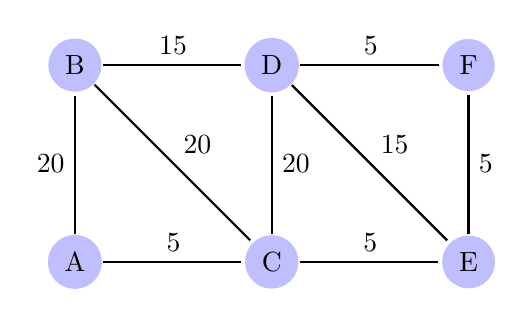
\begin{tikzpicture}[shorten >=1pt,auto,node distance=2.5cm,thick,main node/.style={circle,fill=blue!25}]                      
  \node[main node] (F) {F};                
  \node[main node] (D) [left of=F] {D};    
  \node[main node] (E) [below of=F] {E};   
  \node[main node] (B) [left of=D] {B};    
  \node[main node] (C) [below of=D] {C};   
  \node[main node] (A) [below of=B] {A};   
              
	\path[-, draw, thick]
  (A) edge node {$20$} (B)
	(B) edge node {$20$} (C)
	(B) edge node {$15$} (D)
	(C) edge node[right] {$20$} (D)
	(C) edge node {$5$} (E)
	(D) edge node {$15$} (E)
	(D) edge node {$5$} (F)
	(E) edge node[right] {$5$} (F)
	(A) edge node {$5$} (C)
	;
\end{tikzpicture}

	\caption{Eksempel på en vægtet graf.} \label{fig:weighted_graph}
\end{figure}

TSP er et problem, som netop involverer vægtede grafer. Her søges en kreds af kortest mulig totallængde, der besøger hver knude i en komplet graf præcis én gang.
I Figur \ref{fig:weighted_graph} vil en kreds af kortest mulig længde være $\lbrace A,C \rbrace$, $\lbrace C,E \rbrace$, $\lbrace E,F \rbrace$, $\lbrace F,D \rbrace$, $\lbrace D,B \rbrace$, $\lbrace B,A \rbrace$.
Denne kreds har en længde på $5+5+5+5+15+20=55$.

Dette problem vil projektet undersøge nærmere i Kapitel \ref{chap:TSP}.

